%!TEX root = ../dissertation.tex

\section{Cholinergic Systems}
\newthought{Nary a process in the mammalian body can commence without participation of cholinergic systems.} \Ac{ach} was chemically and pharmacologically described by Henry Dale more than 100 years ago\cite{Dale1914}. A short time later, Otto Loewi published the first proof of signal transmission by small molecules: he transferred physiological solutions from electrically stimulated frog hearts to naive hearts and observed their reactions; the solution that provoked a parasympathetic response he proposed to contain a »vagus substance«\cite{Loewi1921}. Finally, in 1929, Henry Dale completed the picture by isolating acetylcholine from mammalian tissue and identifying it as the molecule responsible for the parasympathetic response\cite{Dale1929}. Dale and Loewi's joint effort in »Discoveries Relating to Chemical Transmission of Nerve Impulses« was rewarded with the »Nobel Prize in Physiology or Medicine« in 1936.

Although we have learned much about cholinergic systems in these past 100 years, our understanding of the mammalian nervous system still is fairly limited. Even when disregarding peripheral nervous systems, the complexity of cholinergic transmission is immense, and a myriad functions have been attributed to cholinergic circuits in the \ac{cns}. Central nervous projections of cholinergic fibres were extensively mapped by M. Marsel Mesulam and others in the 1980s\cite{Mesulam1984}, with a majority of long projection neurons originating in one of the eight cholinergic nuclei, Ch1-Ch8. While many of these anatomical structures have been filled with meaning by associations with both rudimentary as well as higher brain functions, there are still as many cholinergic pathways whose function is entirely unclear (Figure \ref{fig:projections}, from Lobentanzer et al\cite{Lobentanzer2019a}). This holds particularly true for the only recently discovered cortical cholinergic interneurons, which, in comparison to their projecting counterparts, are very small and numerically vastly inferior to other neuron types in the cortex. Thus, their detection and analysis with current methods is challenging. 

\begin{figure}
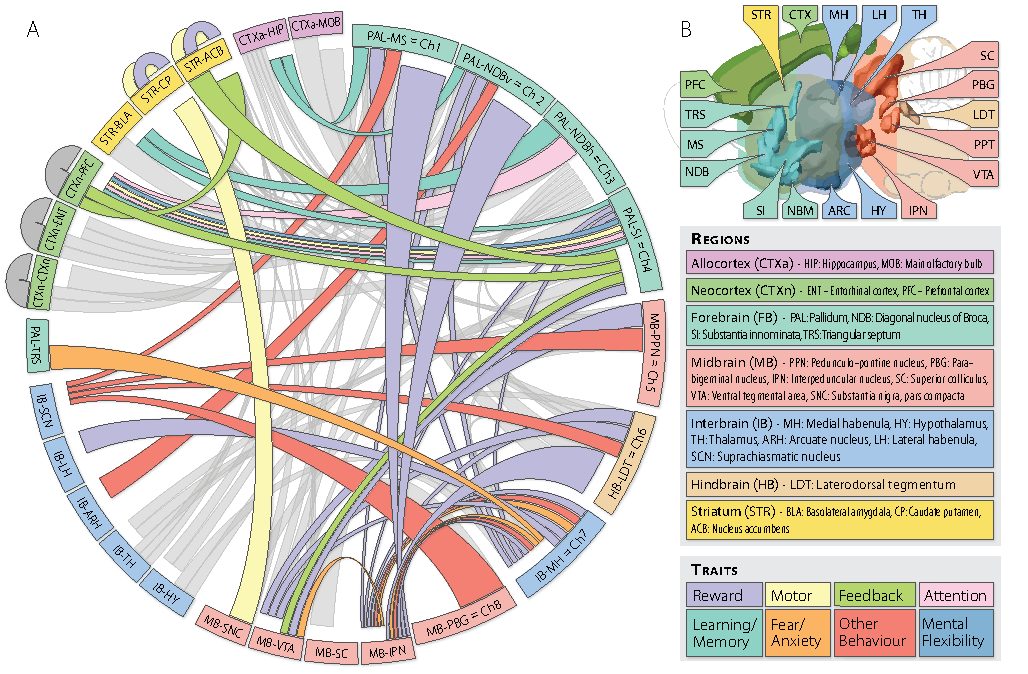
\includegraphics[width=\textwidth]{figures/projections}
\caption[Short figure name.]{This is a figure that floats inline and here is its caption.
\label{fig:projections}}
\end{figure}

Paragraph about cholinergic genes? Box \ref{box:chol-genes}

\begin{mybox}{The Cholinergic Genes}\label{box:chol-genes}
Acetylcholine is generated from acetyl-CoA - supplied by \textbf{ATP citrate lyase} (ACLY) - and choline via enzymatic catalysis by \textbf{choline acetyltransferase}. It is then packed into vesicles by the \textbf{vesicular acetylcholine transporter} (vAChT, SLC18A3). After release into the synaptic cleft, it binds to a variety of \textbf{nicotinic and muscarinic receptors} (CHRN\emph{x}, 16 subunits, and CHRM\emph{x}, 5 subtypes). Of those, the nicotinic receptors form heteropentameric or, seldom, homopentameric ion channels, while the muscarinic receptors are monomeric G protein-coupled transmembrane receptors. The human possesses a duplicate of the nicotinic $\alpha$7 receptor, \textbf{dup$\alpha$7} (CHRFAM7A), which cannot bind ACh and supposedly acts as a dominant negative regulator of the $\alpha$7 homomeric receptor. Termination of the signal is mainly achieved by \textbf{acetylcholinesterase} (ACHE), one of the fastest enzymes known, with a theoretical rate of \num{25000} molecules per second. ACHE tetramers are usually tethered to cell membranes in the synaptic vicinity by the \textbf{proline-rich membrane anchor} (PRIMA1) or \textbf{collagen Q} (COLQ) peptides. Complementary to the mostly residual ACHE is the circulatory \textbf{butyryl cholinesterase} (BCHE), which can also nonspecifically degrade ACh. After degradation, residual choline is reimported into cells via the \textbf{high affinity choline uptake transporter} (HACU, also known as SLC5A7).
\end{mybox}

\subsection{Cholinergic Aspects of Disease} \label{sec:intro:diseases}
\newthought{Cholinergic systems are integral} for a myriad physiological functions, and as such they are critically involved in aetiologies and phenotypes of a number of central and peripheral diseases. Of interest to this dissertation are the cholinergic aspects of degenerative and non-degenerative central nervous diseases (such as Alzheimer's Disease, Bipolar Disorder, Schizophrenia), ischemic conditions in stroke, and peripheral modulation of immune responses, particularly in the context of the aforementioned diseases.

\subsubsection{Alzheimer's Disease}
\ac{ad} was characterised by Alois Alzheimer in 1906 and later named after him by his colleague and mentor, Emil Kraepelin\cite{Berrios1990}. AD is a progressive neurodegenerative disease, its main risk factor is age, and it is estimated to make up 60-70\% of all dementia cases. The disease incidence and progression distinctly differ between the sexes\cite{Miech2002}; generally, women are affected more often. Unlike the very rare familial form (that can affect patients in their fifties), spontaneous AD usually only begins to manifest symptomatically in the 6th to 7th life decade. As a result of the demographic change in most western countries, patient numbers, and thus, medical efforts, are expected to more than double in size until the year 2050. The cognitive decline associated with AD is progressive and ultimately leads to exhaustive care dependency; there is no cure.

The pathological hallmarks of AD are two types of atypical protein aggregates, inter-cellular amyloid $\beta$ »plaques«, and intra-cellular »neurofibrillary tangles« composed of hyper-phosphorylated tau-protein. Often, pathological aggregation of these proteins begins decades before the onset of symptoms. However, there have also been numerous cases of cognitively healthy subjects showing high amounts of protein aggregates. These inconsistencies and the unclear causality of pathology and symptoms have led to a redirection of scientific efforts to processes unrelated to amyloid and tau, such as neuroinflammation.

Cholinergic systems have long been associated with AD, as evidenced by the cholinergic hypothesis that was posed in the 1980s. To cite from Bartus et al, 1982\cite{Bartus1982}:

\begin{quote}
»We have been guided by three deductive requirements that must be satisfied if the cholinergic hypothesis is to deserve continued attention: (i) specific dysfunctions in cholinergic markers should be found in the brains of subjects suffering from age-related memory loss, (ii) artificial disruption of central cholinergic function in young subjects should induce behavioural impairments that mimic the cognitive loss found naturally in aged subjects, and (iii) appropriately enhancing central cholinergic activity in aged subjects should significantly reduce age-related cognitive deficits.«
\end{quote}

Although many reports substantiate all three deductive prerequisites, the cholinergic hypothesis has in the last decades been overshadowed by alternative hypotheses, particularly, amyloid-related theories. However, the therapeutic approaches developed along the line of preventing amyloid $\beta$ aggregation or otherwise clearing the plaques or soluble aggregates have not been successful in alleviating the cognitive decline in patients(cite). Thus, pro-cholinergic intervention by means of \ac{ache} inhibition still makes up the majority of approved drugs. The monotherapeutic approach of ACHE inhibition is based on a premise that seems simple in light of the enormous complexity surrounding the interplay of the billions of neurons in the process of memory formation and recall, and in fact, pro-cholinergic therapy has only been shown to alleviate symptoms or delay their onset; a reversal of cognitive losses has so far not been achieved by any drug regime. As such, even in regard only to the cholinergic systems, novel approaches are sorely needed.

On the other hand, the cholinergic deficit in AD is not purely symptomatic. There is considerable debate whether the pathology originates from the entorhinal cortex or the basal forebrain. As Heiko and Eva Braak have shown\cite{Braak1995}, AD pathology follows a characteristic brain region distribution process that can be stratified into stages and starts in the entorhinal region. The early stages of pathology by far precede the onset of symptoms. Newest longitudinal \emph{in vivo} imaging studies now substantiate the cholinergic origin of neurodegeneration: In cognitively normal and impaired human subjects, basal forebrain volume predicted longitudinal entorhinal degeneration, but not \emph{vice versa}. As such, the cholinergic basal forebrain dysfunction precedes as well as predicts pathology in other affected areas and cognitive deficits\cite{Schmitz2016}.

% sexual dimorphism in response to ache inhibitors Giacobini2018

\subsubsection{Schizophrenia and Bipolar Disorder}
Cognitive deficits can also occur without neuron death. The earliest description of what we today call \ac{scz} was coined by Emil Kraepelin: »\emph{dementia praecox}«, premature dementia\cite{Kraepelin1913}. Cognitive deficits are an integral but often overlooked part of the clinical picture of SCZ, which is often dominated by the more impressive positive symptoms such as hallucinations and paranoia. Likewise, \ac{bd} can present with cognitive impairments. The cognitive impairments affecting both SCZ and BD patients involve diminished problem solving capabilities and reduced intelligence, and are more pronounced in SCZ than in BD\cite{Bortolato2015}. They have been connected to cholinergic dysfunction\cite{VanEnkhuizen2015, Smucny2017} and the sum of anticholinergic medications\cite{Gray2015, Eum2017}. A human polymorphism in the $\alpha$5 nicotinic receptor subunit predicts a higher propensity for smoking and SCZ, showing parallel manifestations in engineered mice\cite{Koukouli2017} and rats\cite{Forget2018}. Correspondingly, cholinergic stimulation can improve cognition\cite{Sacco2004, Rowe2015, Lewis2017} and mood\cite{Higley2014}, but can on the other hand provoke schizotypic behaviour in AD patients\cite{Degirmenci2016}.

SCZ and BD clinically present with clear sexual dimorphisms. Compared to women, men have a higher SCZ prevalence with an \ac{or} of 1.4, are affected earlier (at 15-25 as compared to 25-35 years of age), and face a worse prognosis\cite{Leger2016}. Cholinergic participation also appears sex-dependent: Male SCZ patients more often self-medicate by smoking (7.2 versus 3.3 weighted average OR with 90\% lifetime prevalence)\cite{DeLeon2005}. BD, on the other hand, affects men and women almost equally (OR $\smallsim$\num{1}). However, women make up 80-90\% of so-called »rapid cyclers«, a subgroup of patients showing short intervals between manic and depressive phases which is associated with a worse prognosis\cite{Berger2014}. Additionally, major depressive disorder, which is a prerequisite for BD diagnosis, more often affects women\cite{Berger2014} (OR = 2).

Psychiatric genomics has recently identified a high amount of shared heritability between SCZ and BD\cite{Anttila2018}. Likewise, transcriptomic analyses have shown a high correlation (71\%) between the transcriptional perturbations in the two diseases. Clinical as well as molecular pathology intensifies from BD to SCZ, suggesting the two lie on different points of a shared spectrum. However, their genetic origins are tremendously complex. Multiple disease-relevant markers have been identified by GWAS (genome-wide association studies), even able to distinguish between several sub-phenotypes of each disease\cite{Ruderfer2018}. These markers are found in neurotransmitter receptors (e.g., dopaminergic, glutamatergic, cholinergic), scaffolding proteins (DISC: »disrupted in schizophrenia«), multiple \acp{tf}, \acp{mir}, and non-coding regions without known function\cite{Harrison2015, Henriksen2017, Kanazawa2017}.

Considering this complex disease aetiology, it is not surprising that there are no »designer« drugs available against SCZ and BD. All available therapeutic options have been empirically found, starting with the first antipsychotic, chlorpromazine, synthesised in 1950 by the French pharmaceutical company Rhône-Poulenc. Originally developed in a series dedicated to the search for antihistaminics, it was soon recognised for its antipsychotic potential, and widely prescribed only few years later. Many other neuroleptic compounds have been derived from chlorpromazine, and through binding affinity assays, their receptor profiles were established. Most compounds with antipsychotic properties have a wide spectrum of different receptor activities, but most early drugs were strong antagonists of the D$_2$ dopamine receptor. Thus, the »dopaminergic hypothesis« of SCZ was formulated. However, aetiology as well as therapeutic principles are unclear to this day, and most antipsychotic substances still are very »dirty drugs«. In fact, newer developments leading to the discovery of the second generation (»atypical«) neuroleptic substances, starting with clozapine, have created molecules with an even wider spectrum of interactions und thus less specificity towards a single therapeutic mechanism of action. This development is contrary to pharmaceutical research practice, where most developments aim for a higher specificity.

\subsubsection{Immunity}
Aside from its vast neuronal functions, \ac{ach} also is highly relevant in immune cells. The first to isolate ACh from an animal organ, Dale and Dudley\cite{Dale1929}, used the spleens of oxen and horses. The spleen receives sympathetic, but not parasympathetic innervation, and as such, the ACh found by Dale and Dudley had to have come from immune cells. Indeed, nearly all mammalian immune cells express cholinergic components, most importantly, B- and T-cells, macrophages, and dendritic cells\cite{Fujii2017}. ACh is physico-chemically as well as enzymatically unstable, and thus has to be supplied synaptically or, at most, in paracrine fashion. Soluble esterases cleave ACh with stunning efficiency, reducing its diffusion range to few millimetres. \ac{chat} activity has been confirmed in B- and T-cells, which both contain significant amounts of ACh, although T-cells generally possess higher amounts. Additionally, in peripheral cells ACh can be synthesised by the mitochondrial carnitine acetyltransferase. In addition to B- and T-cells CHAT mRNA has been found in macrophages and dendritic cells. CHAT expression and ACh synthesis can be activated by various immune mediators, such as lipopolysaccharides and toll-like receptor agonists.

In addition to ACh synthesis, all of the aforementioned cell types can receive cholinergic signals. They express all muscarinic receptors as well as a selection of nicotinic receptor subunits, and the signal-terminating esterases.

\subsubsection{Stroke}
Stroke is a medical emergency in which reduced blood flow leads to massive neuron death in the brain. There are two types of stroke: Haemorrhagic stroke, which is caused by bleeding due to a rupture of brain vessels, and ischemic stroke, misperfusion of a brain region caused by a clot in a cranial artery. Ischemic stroke makes up the vast majority of all strokes, about 90\%. Stroke is currently responsible for the second most frequent cause of death in developed countries, only second to coronary artery disease. Those who survive the stroke are in many cases permanently and severely disabled.

\subsection{Neurokines} \label{sec:intro:neurokine}
In comparison to the widely studied cholinergic projection neurons originating in the basal forebrain (Ch1-Ch4) that are known to depend on a retrograde survival signal by means of \ac{ngf}, trophic influences on other cholinergic populations such as the cortical interneurons are unclear.  \ac{ngf} was described by Rita Levi-Montalcini in the 1950s as the first known instance of trophic peptides required for the survival of sympathetic ganglia\cite{Levi-Montalcini1960}. The group of neurotrophic substances since discovered (most prominently, the brain-derived neurotrophic factor \acs{bdnf}) are commonly referred to as »neurotrophins«. They convey their trophic effects through a family of transmembrane receptors; NGF binds to \ac{ntrk1} with high affinity, BDNF binds to \ac{ntrk2} with high affinity. However, both also bind to a third receptor, \ac{ngfr}, which is also known as p75, although with low affinity. NGFR function is complex, depending on the context it seems to be able to suppress as well as enhance the primary neurotrophic signal mediated by NTRK1/2(cite). The dependence of basal forebrain cholinergic neurons on retrograde NGF signalling was discovered in the 1980s\cite{Hefti1986}.  

A second group of trophic peptides with cholinergic implications are the so-called »neurokines«; the name results from the fact that this particular subgroup of cytokines has been associated with neuronal function in the central and peripheral nervous systems. Most prominently they include the \ac{cntf}, \ac{lif}, and \ac{il}, all of which coincidentally have been known under the acronym CDF. In the end of the 1980s, two groups of scientists (McManaman\cite{McManaman1988} and Rao\cite{Rao1992}) independently identified proteins in extracts of muscle fibre that induced a differentiation of neurons towards a cholinergic type, and thus termed these proteins »choline acetyltransferase development factor« or »cholinergic differentiation factor« (both abbreviated CDF). Only later, through sequencing of the peptides, it became known that they had in fact discovered two distinct neurokines, \ac{lif} (Rao) and \ac{cntf} (McManaman, personal communication). \ac{il}, on the other hand, is abbreviated CDF for an entirely different reason: in this case it is short for »CTL (cytolytic T lymphocyte) differentiation factor«.

\ac{cntf}, \ac{lif}, and \ac{il} convey their impact on neuronal activity through a partly redundant neurokine receptor pathway\cite{Berger2014}. There are two basic types of neurokine receptors: soluble and transmembrane. The primary receptors for \ac{cntf} (\acs{cntfr}) and \ac{il} (\acs{ilr}) are soluble proteins that are secreted into the extracellular space and, upon binding of a neurokine, bind to transmembrane receptor dimers on the cell surface. These transmembrane receptors are the LIF receptor (\acs{lifr}) and the »interleukin 6 signal transducer« (\acs{ilst}, also known as \acs{gp}). Every neurokine has its preferred constellation of soluble and transmembrane receptors: \ac{cntf} binds to the soluble \ac{cntf} receptor and a dimer consisting of one \ac{gp} and one \ac{lifr} protein; \ac{il} binds to the soluble IL6R and a dimer of two units of \ac{gp}; \ac{lif} does not usually bind a soluble receptor but rather binds immediately to a dimer comprising one of each \ac{gp} and \ac{lifr}; however, there is significant redundancy and crosstalk between those systems\cite{Rawlings2004,Nathanson2012}.

All receptor constellations result in a main effect of activation of the \acs{jak}/\acs{stat} cascade (Fig.\,\ref{fig:neurokine}). More specifically, neurokines can activate \acfp{jak} 1 and 2 or the homologous \ac{tyk} 2, and, successively, \ac{stat} (»signal transducer and activator of transcription«) isoforms 1, 3, 5A, and 5B, which then convey a multitude of cellular effects (e.g. in immunity or differentiation) through transcriptional activation. The \ac{stat} cascade is inherently self-limiting in that it usually leads to expression of transcription factors that serve as repressors of the \ac{stat} genes (XXX)\cite{}. 

Neurokines, particularly \ac{il}(?), might serve as a link between the immunological and cholinergic aspects of physiological or disease processes.\todo{elaborate}

\begin{figure}
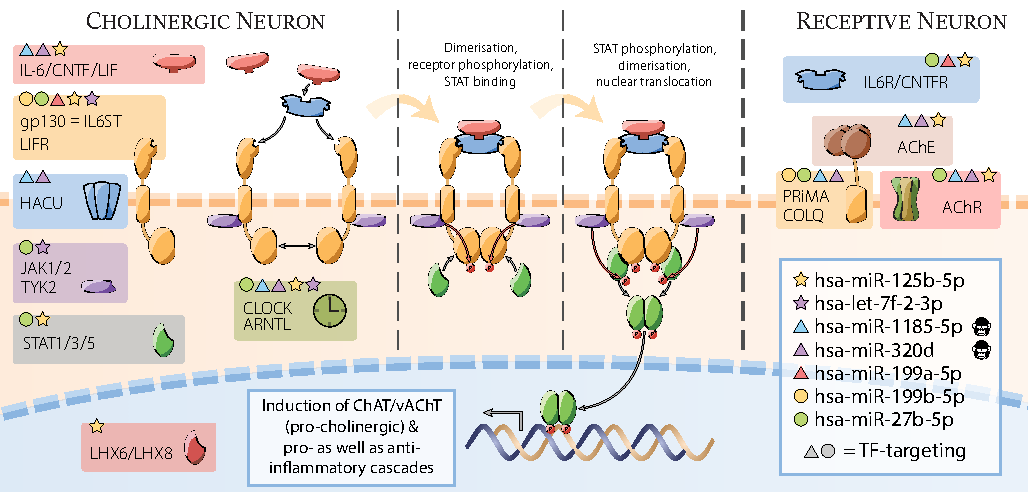
\includegraphics[width=\textwidth]{figures/neurokine}
\caption[Short figure name.]{This is a figure that floats inline and here is its caption.
\label{fig:neurokine}}
\end{figure}

%Neuronal activity is profoundly modified by cytokines

%Li Gan - NFkB activation by tau
% - Ikkbeta knockout corrects STAT1 DE

%Oleg Butovsky - TGFbeta as master glia regulator